% 2015-07-16 - Matthew A. Wolff - Thesis research presentation

\documentclass{beamer}

\mode<presentation> {
	% Themes and color schemes:
	\usetheme{default}
	\usecolortheme{rose}
}

% Need this on campus machine (but not at home)
%\usepackage{sansmathaccent}
%\pdfmapfile{+sansmathaccent.map}

\usepackage{graphicx} % Allows including images
\usepackage{booktabs} % Allows the use of \toprule, \midrule and \bottomrule in tables

%------------------------------------------------------------------------------
%	TITLE PAGE
%------------------------------------------------------------------------------

% The short title appears at the bottom of every slide, the full title is only on the title page
\title[Multilevel Summation Method]{Multilevel Summation Method} 

\author{Matthew A. Wolff} % Your name
\institute[Purdue University] % Your institution as it will appear on the bottom of every slide, may be shorthand to save space
{
	Purdue University \\ % Your institution for the title page
	\medskip
	\textit{wolff1@purdue.edu} % Your email address
}
\date{July 17, 2015} % Could also use \today, if desired

% Add slide numbers
\setbeamerfont{page number in head/foot}{size=\small}
\setbeamertemplate{footline}[frame number]

\begin{document}

\begin{frame}
	\titlepage % Print the title page as the first slide
\end{frame}

\begin{frame}
	\frametitle{Overview} % Table of contents slide, comment this block out to remove it
	\tableofcontents % Throughout your presentation, if you choose to use \section{} and \subsection{} commands, these will automatically be printed on this slide as an overview of your presentation
\end{frame}

%*-*-*-*-*-*-*-*-*-*-*-*-*-*-*-*-*-*-*-*-*-*-*-*-*-*-*-*-*-*-*-*-*-*-*-
%* MSM with Single Splitting
%*-*-*-*-*-*-*-*-*-*-*-*-*-*-*-*-*-*-*-*-*-*-*-*-*-*-*-*-*-*-*-*-*-*-*-
\section{Single Splitting}

\frame{
	\frametitle{What?, Why?, When?, Where?, How?}
	\begin{itemize}
		\item What: Split the kernel once
		\item Why: The term which is interpolated has infinite extent
		\item When: Explicitly when forming the algorithm
		\item Where: The long-range part of the kernel
		\item How: This will be the focus of today's presentation
	\end{itemize}
}

\frame{
	\frametitle{What?}

	Split the computational kernel once:
	\begin{itemize}
		\item $k(\textbf{r},\textbf{r}') = \frac{1}{\| \textbf{r}' - \textbf{r} \|}$
		\item $k(\textbf{r},\textbf{r}') = k_0(\textbf{r},\textbf{r}') + k_1(\textbf{r},\textbf{r}')$
		\begin{itemize}
			\item "Short-range" component, $k_0$, is computed exactly via geometric hashing
			\item "Long-range" component, $k_1$, is interpolated on a hierarchy of grids
		\end{itemize}
	\end{itemize}
}

\frame{
	\frametitle{Why?}

	In general, interpolation using B-Splines can be shown to have the form:
	\[ \bar{f}(x) = \sum_n{f_n^\ell\phi_n^\ell(x)} \]
	where
	\begin{itemize}
		\item $\bar{f}(x)$ is the interpolant
		\item $f_m^\ell = \sum_n{\omega_{m-n}f(nh_\ell)}$
		\item $f(x)$ is continuous, bounded objective function
		\item $\phi_n^\ell(x) = \Phi(x/h_\ell - n)$
	\end{itemize}

	\vspace{0.2in}

	So, single-split because
	\begin{itemize}
		\item B-Spline interpolant of a function with compact support is not compact
%		\item FIXME: pic of exaggerated function and interpolant
		\item Long-range component does not have compact support
	\end{itemize}
}

\frame{
	\frametitle{How?}

	Algorithmic overview:
	\begin{itemize}
		\item Interpolate function, $f(x)$, on coarsest grid, $\Omega^L$
		\item Compute interpolation error, $\Delta^{L-1}(x)$, on next finest grid, $\Omega^{L-1}$, at coarse-grid points and mid-points
		\item Do:
		\begin{itemize}
			\item If $ \| \Delta^\ell(x) \| \leq \tau $, then exit loop
			\item Else, interpolate $\Delta^\ell(x)$ on $\Omega^\ell$
			\item Compute updated interpolation error, $\Delta^{\ell-1}$, on next finest grid, $\Omega^{\ell-1}$, at points and midpoints of $\Omega^\ell$
			\item Set $\ell = \ell - 1$
			\item Repeat
		\end{itemize}
	\end{itemize}
}

\frame{
	\frametitle{How? - Example}	% f(x)
	\begin{center}
		\mbox{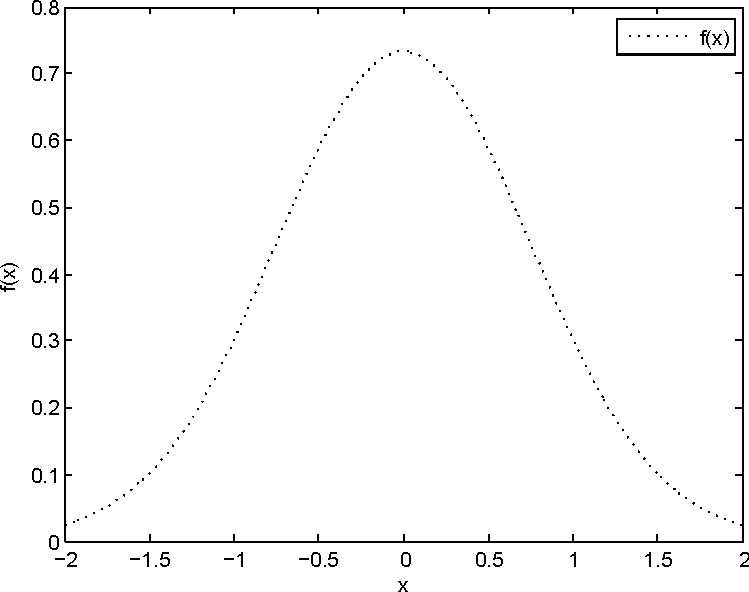
\includegraphics[width=0.9 \textwidth]{../Figures/Refine1.pdf}}
	\end{center}
	\[ \text{ }  \]
}

\frame{
	\frametitle{How? - Example}	% f(x), f_1(x)
	\begin{center}
		\mbox{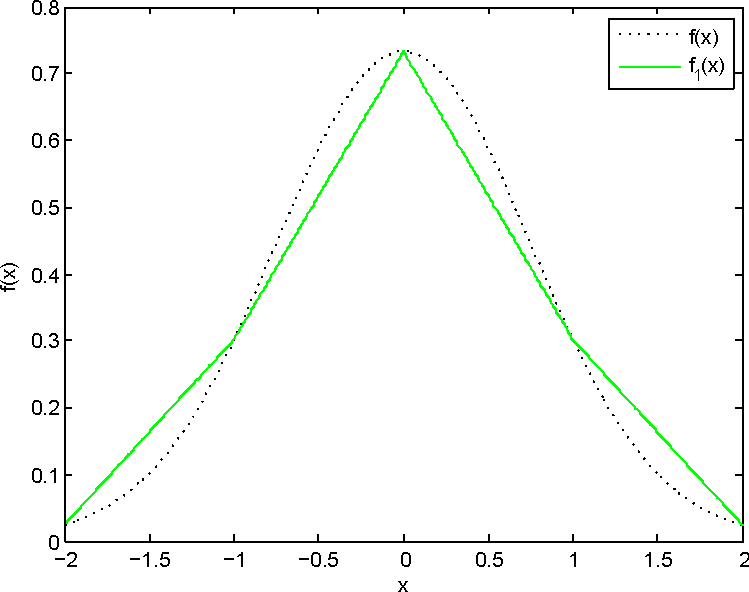
\includegraphics[width=0.9 \textwidth]{../Figures/Refine2.pdf}}
	\end{center}
	\[ f(x) \approx \textcolor{green}{f_1(x)}  \]
}

\frame{
	\frametitle{How? - Example}	% f(x), f_1(x), f_2(x)
	\begin{center}
		\mbox{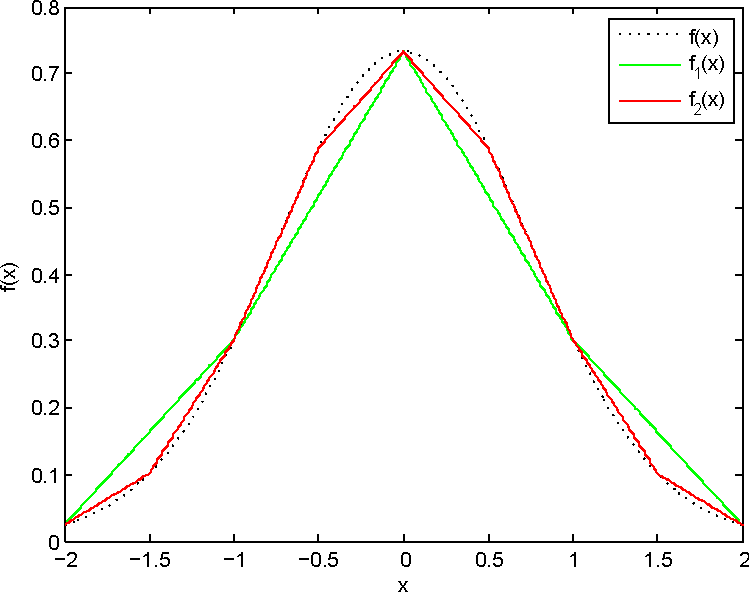
\includegraphics[width=0.9 \textwidth]{../Figures/Refine3.pdf}}
	\end{center}
	\[ f(x) \approx \textcolor{red}{f_2(x)} = \textcolor{green}{f_1(x)} + \Delta^2(x) \]
}

\frame{
	\frametitle{How? - Example}	% f(x), f_1(x), f_2(x), f_3(x)
	\begin{center}
		\mbox{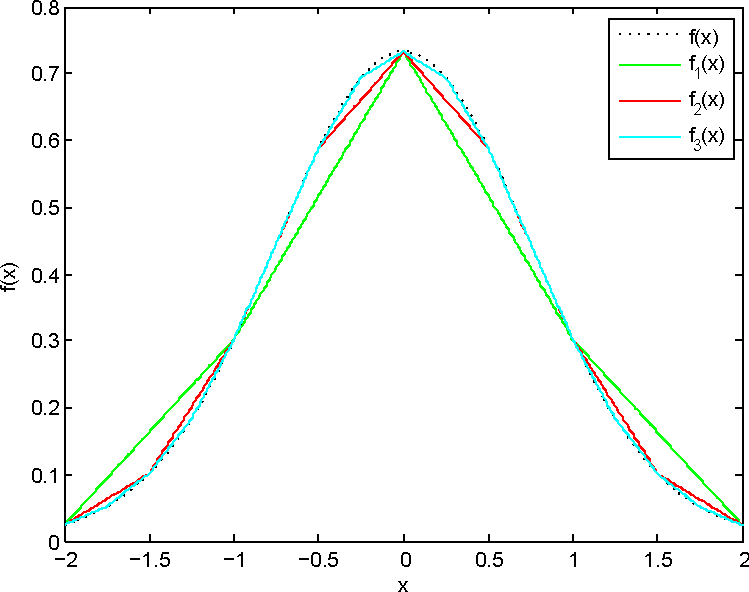
\includegraphics[width=0.9 \textwidth]{../Figures/Refine4.pdf}}
	\end{center}
	\[ f(x) \approx \textcolor{cyan}{f_3(x)} = \textcolor{green}{f_1(x)} + \textcolor{red}{\Delta^2(x)} + \Delta^3(x) = \textcolor{red}{f_2(x)} + \Delta^3(x)  \]
}

\frame{
	\frametitle{How? (Continued)}
	Currently, two main questions:
	\begin{enumerate}
		\item How to compute stencils?
		\item How to remove basis functions?
	\end{enumerate}
}

\subsection{How to compute stencils?}

\frame{
	\frametitle{How to compute stencils?}
	Define the following:
	\begin{itemize}
		\item $f(x)$ is objective function
		\item $\bar{f}^\ell(x)$ is interpolant of $f(x)$ using grids $\Omega^\ell$ through $\Omega^L$
		\item $\Delta^\ell(x)$ is interpolation error of $\bar{f}^{\ell+1}$
		\begin{itemize}
			\item $\Delta^\ell(x) = f(x) - \bar{f}^{\ell+1}$
		\end{itemize}
		\item $\hat{\Delta}^\ell(x)$ is anti-blurred $\Delta^\ell(x)$ (i.e. stencil of coefficients)
		\begin{itemize}
			\item $\hat{\Delta}^\ell(x) = \mathcal{A} \Delta^\ell(x)$
		\end{itemize}
		\item $\bar{\Delta}^\ell(x)$ is interpolant of $\Delta^\ell(x)$
		\begin{itemize}
			\item $\bar{\Delta}^\ell(x) = \mathcal{B} \mathcal{A} \Delta^\ell(x)$
		\end{itemize}
	\end{itemize}
	
	Then, using the coarsest $\ell$ grids, the interpolant is given by
	\[ \bar{f}^\ell(x) = \bar{f}^L(x) + \bar{\Delta}^{L-1}(x) + \dots + \bar{\Delta}^{\ell+1}(x) + \bar{\Delta}^\ell(x) = \bar{f}^{\ell+1} + \bar{\Delta}^\ell(x) \]
}

\subsection{How to remove basis functions?}

\frame{
	\frametitle{How to remove basis functions?}

%	\begin{itemize}
%		\item Which basis function(s) \it{can} be removed?
%	\end{itemize}
	Rearrange terms in interpolant as follows:
	\[ \bar{f}^\ell(x) = \bar{f}^{\ell+} + \bar{f}^{\ell-}  \]
	where
	\begin{itemize}
		\item $\bar{f}^{\ell+}$ are terms with \textbf{required} basis functions
		\item $\bar{f}^{\ell-}$ are terms with \textbf{unnecessary} basis functions
	\end{itemize}

	Now, we have:
	\begin{align}
		f(x) &= \bar{f}^\ell(x) + \Delta^{\ell-1} \\
		&= \bar{f}^{\ell+} + \bar{f}^{\ell-} + \Delta^{\ell-1}
	\end{align}
	
	and we want to stop at level $\ell$ when
	\begin{align}
		\| f(x) - \bar{f}^{\ell+}(x) \| &\leq \tau \\
		\| \bar{f}^{\ell-} + \Delta^{\ell-1} \| &\leq \tau
	\end{align}
}

%\section{Roadmap to completion}
%
%\frame{
%	\frametitle{Roadmap to Completion}
%	Overview:
%	\begin{itemize}
%		\item Single-split MSM
%		\begin{itemize}
%			\item Update pre-processing to build stencil for each grid level
%			\item Force evaluation code largely unaffected
%			\begin{itemize}
%				\item Update direct calculation routine to use stencil-specific radius
%			\end{itemize}
%			\item Compare accuracy to multi-split version
%		\end{itemize}
%	\end{itemize}
%}

\section{Conclusion}

\frame{
	\frametitle{Conclusion}

	Need to
	\begin{itemize}
		\item Find $\bar{f}^{\ell-}$ and round those coefficients to zero
		\item Find optimal way to do this for minimal computational complexity
	\end{itemize}
}

%\frame{
%	\frametitle{The end}
%	\begin{center}
%		Thank you!
%	\end{center}
%}

%\frame{
%	\frametitle{Bibliography}
%	\begin{itemize}
%		\item \tiny{A. Brandt and A. Lubrecht, \textit{Multilevel Matrix Multiplication and Fast Solution of Integral Equations}, J. Comp. Phys., 90 (1990), pp. 348-370.}
%		\item \tiny{A. Brandt and C. Venner, \textit{Multilevel Evaluation of Integral Transforms with Asympotically Smooth Kernels}, SIAM J. Sci. Comput., Vol. 19, No. 2 (1998), pp. 468 - 492.}
%		\item \tiny{D. Hardy. \textit{Multilevel Summation for the Fast Evaluation of Forces for the Simulation of Biomolecules}. PhD thesis, Univ. of Illinois at Urbana-Champaign, 2006.}
%		\item \tiny{M. Griebel, S. Knapek, and G. Zumbusch, \textit{Numerical simulation in molecular dynamics}, Springer (2007).}
%		\item \tiny{D. Hardy, J. Stone, and K. Schulten, \textit{Multilevel summation of electrostatic potentials using graphics processing units}, Parallel Computing, 35 (2009), pp. 164 - 177.}
%		\item \tiny{S. Moore and P. Crozier, \textit{Extension and evaluation of the multilevel summation method for fast long-range electrostatics calculations}, J. Chem. Phys., 140 (2014), pp. 234112-1 - 234112-12.}
%		\item \tiny{D. Tameling, P. Springer, P. Bientinesi, and A. Ismail, \textit{Multilevel summation for dispersion: A linear time algorithm for $r^{-6}$ potentials}, J. Chem. Phys., 140 (2014), pp. 024105-1 - 024105-12.}
%		\item \tiny{D. Hardy, M. Wolff, J. Xia, K. Schulten, R. Skeel, \textit{Multilevel Summation Using B-Spline Interpolation}, In preparation (2015).}
%	\end{itemize}
%}

\end{document}